\chapter{Flowers, Fruits and Seeds}\label{ch:g3:flowers-fruits-seeds}

In April the cherry tree is white with blossom; in June it hangs
with cherries. Where did the \omterm{def:g3:flowers-fruits-seeds:parts}{flowers} go --- and where did the
\omterm{prop:g3:flowers-fruits-seeds:transform}{fruit} come from? The answer is one of the prettiest
transformations in the living world: the \omterm{def:g3:flowers-fruits-seeds:parts}{flower} does not
disappear, it \emph{becomes} the \omterm{prop:g3:flowers-fruits-seeds:transform}{fruit}.

\section{Looking inside a flower}

\begin{definition}[The parts of a flower]\label{def:g3:flowers-fruits-seeds:parts}
A \emph{flower}\index{flower} is the part of the \omterm{def:g1:plants-around-us:plant}{plant} that will
make the \omterm{prop:g3:flowers-fruits-seeds:transform}{seeds}. From the outside in:
\begin{enumerate}
  \item the \emph{petals}\index{petal}, colored and scented, which
        attract visiting \omterm{prop:g3:sorting-living-things:groups}{insects};
  \item the \emph{stamens}\index{stamen}, thin stalks dusted with
        \emph{pollen}\index{pollen}, a fine yellow powder;
  \item in the very center, the \emph{pistil}\index{pistil}, a
        little flask; deep inside it lie the flower's future
        \omterm{prop:g3:flowers-fruits-seeds:transform}{seeds}.
\end{enumerate}
\end{definition}

\begin{omfigure}
\begin{tikzpicture}
  \node[anchor=south west, inner sep=0] (img) at (0,0)
    {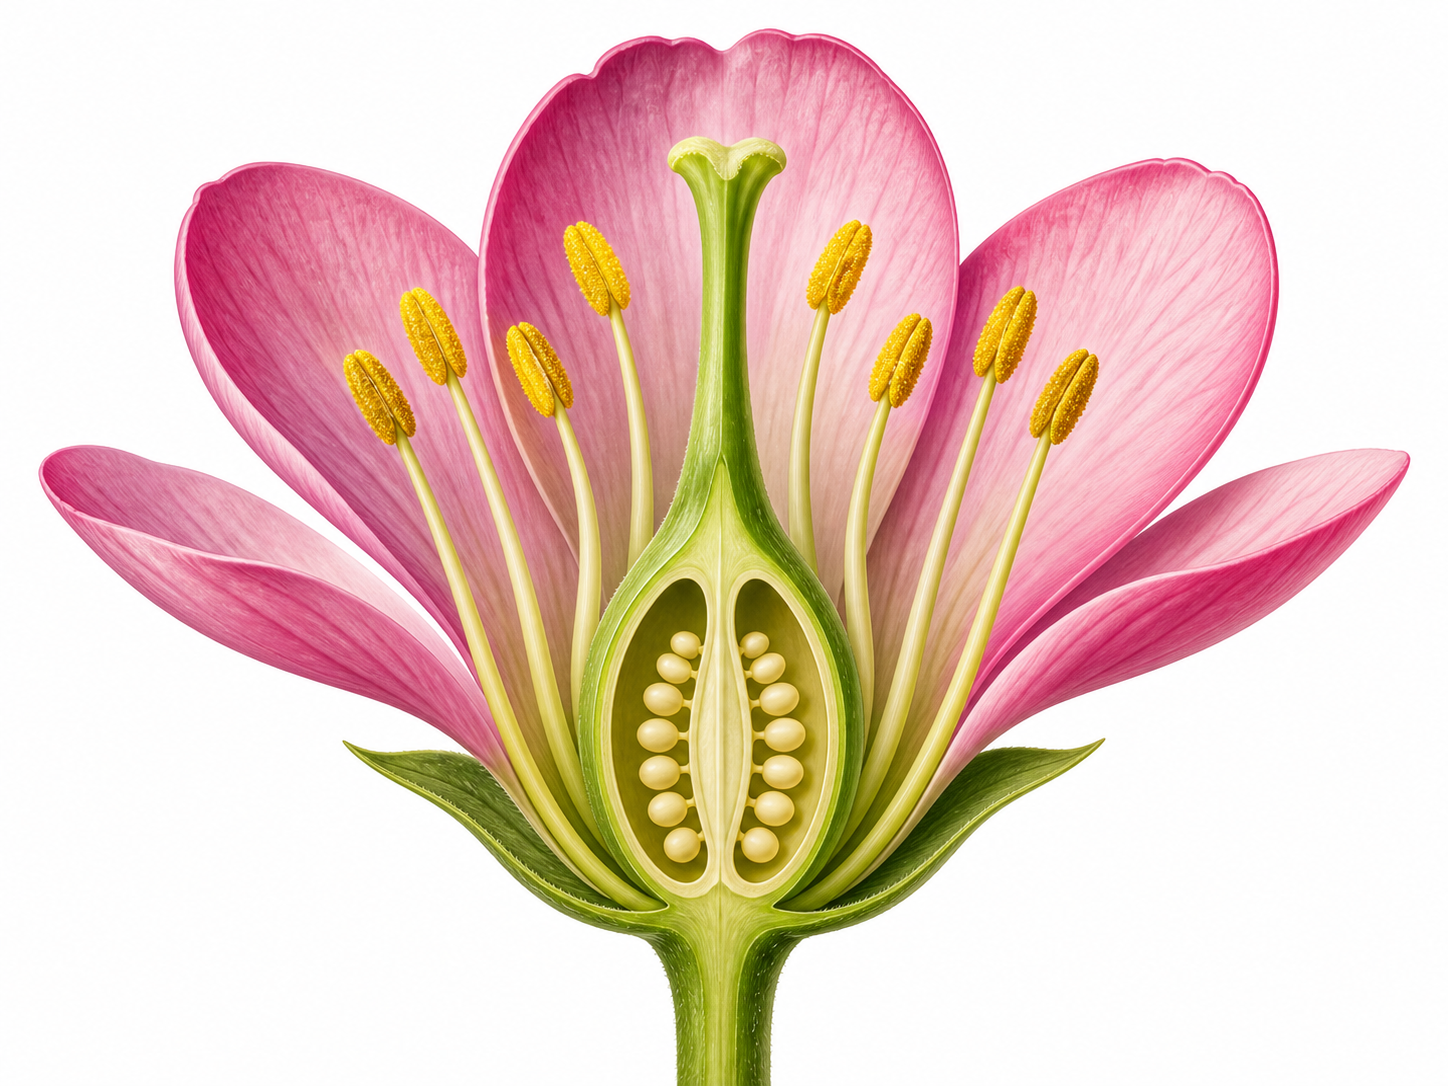
\includegraphics[width=0.6\linewidth]{images/book1/ai/fig-flower-cutaway.png}};
  \begin{scope}[x={(img.south east)}, y={(img.north west)},
      every node/.style={font=\small}]
    \draw[omDef, thick] (0.82,0.80) -- (0.93,0.90) node[above] {petal};
    \draw[omDef, thick] (0.72,0.68) -- (1.03,0.66)
      node[right, align=left] {stamen, dusted\\ with pollen};
    \draw[omDef, thick] (0.56,0.36) -- (1.03,0.34)
      node[right, align=left] {pistil: the future\\ seeds are inside};
    \draw[omDef, thick] (0.505,0.05) -- (0.66,0.04) node[right] {stem};
  \end{scope}
\end{tikzpicture}

{\small Inside a \omterm{def:g3:flowers-fruits-seeds:parts}{flower}, cut in half: \omterm{def:g3:flowers-fruits-seeds:parts}{petals} around, pollen-bearing
\omterm{def:g3:flowers-fruits-seeds:parts}{stamens}, and the \omterm{def:g3:flowers-fruits-seeds:parts}{pistil} in the center with the future \omterm{prop:g3:flowers-fruits-seeds:transform}{seeds} inside.}
\end{omfigure}

\begin{example}[Dissecting a tulip]\label{ex:g3:flowers-fruits-seeds:tulip}
Open a wilting tulip gently, \omterm{def:g3:flowers-fruits-seeds:parts}{petal} by \omterm{def:g3:flowers-fruits-seeds:parts}{petal}. Inside stand the
\omterm{def:g3:flowers-fruits-seeds:parts}{stamens} --- brush one on your finger and it \omterm{def:g1:plants-around-us:parts}{leaves} yellow \omterm{def:g3:flowers-fruits-seeds:parts}{pollen}
dust --- and in the middle the fat green \omterm{def:g3:flowers-fruits-seeds:parts}{pistil}. Slice the \omterm{def:g3:flowers-fruits-seeds:parts}{pistil}
across (a grown-up's knife-work) and there they are: rows of
tiny pale future \omterm{prop:g3:flowers-fruits-seeds:transform}{seeds}.
\end{example}

\section{From flower to fruit}

\begin{proposition}[Pollination, then transformation]\label{prop:g3:flowers-fruits-seeds:transform}
For the transformation to start, \omterm{def:g3:flowers-fruits-seeds:parts}{pollen} must reach the \omterm{def:g3:flowers-fruits-seeds:parts}{pistil} ---
that step is \emph{pollination}\index{pollination}. Bees and
other \omterm{prop:g3:sorting-living-things:groups}{insects} do most of the carrying, dusted with \omterm{def:g3:flowers-fruits-seeds:parts}{pollen} as they
drink from \omterm{def:g3:flowers-fruits-seeds:parts}{flower} after \omterm{def:g3:flowers-fruits-seeds:parts}{flower}; the wind does some too. After
pollination:
\begin{itemize}
  \item the \omterm{def:g3:flowers-fruits-seeds:parts}{petals} and \omterm{def:g3:flowers-fruits-seeds:parts}{stamens}, their work done, wither and fall;
  \item the \omterm{def:g3:flowers-fruits-seeds:parts}{pistil} swells and becomes the
        \emph{fruit}\index{fruit};
  \item the future \omterm{prop:g3:flowers-fruits-seeds:transform}{seeds} inside it become the
        \emph{seeds}\index{seed}.
\end{itemize}
A \omterm{prop:g3:flowers-fruits-seeds:transform}{fruit} is a transformed \omterm{def:g3:flowers-fruits-seeds:parts}{pistil}, and every true \omterm{prop:g3:flowers-fruits-seeds:transform}{fruit} carries
\omterm{prop:g3:flowers-fruits-seeds:transform}{seeds}.
\end{proposition}
\admitted

\begin{example}[Watching one cherry happen]\label{ex:g3:flowers-fruits-seeds:cherry}
Follow a single cherry blossom. April: white \omterm{def:g3:flowers-fruits-seeds:parts}{petals}, buzzing
bees. May: \omterm{def:g3:flowers-fruits-seeds:parts}{petals} snowing down; where each \omterm{def:g3:flowers-fruits-seeds:parts}{flower} stood, a tiny
green ball --- the swelling \omterm{def:g3:flowers-fruits-seeds:parts}{pistil}. June: the ball grown red and
sweet --- a cherry, with the stone (its \omterm{def:g2:from-seed-to-plant:seed}{seed}) inside. The \omterm{def:g3:flowers-fruits-seeds:parts}{flower}
did not fall; only its \omterm{def:g3:flowers-fruits-seeds:parts}{petals} did.
\end{example}

\begin{remark}[No bees, no cherries]\label{rem:g3:flowers-fruits-seeds:bees}
Cherry growers welcome beekeepers' hives into their orchards ---
without insect visits, most blossoms would stay unpollinated and
fall without ever becoming \omterm{prop:g3:flowers-fruits-seeds:transform}{fruit}. The bee is not stealing from
the \omterm{def:g3:flowers-fruits-seeds:parts}{flower}; \omterm{def:g3:flowers-fruits-seeds:parts}{flower} and bee feed each other: nectar for the bee,
\omterm{def:g3:flowers-fruits-seeds:parts}{pollen} delivery for the \omterm{def:g1:plants-around-us:plant}{plant}.
\end{remark}

\begin{omfigure}
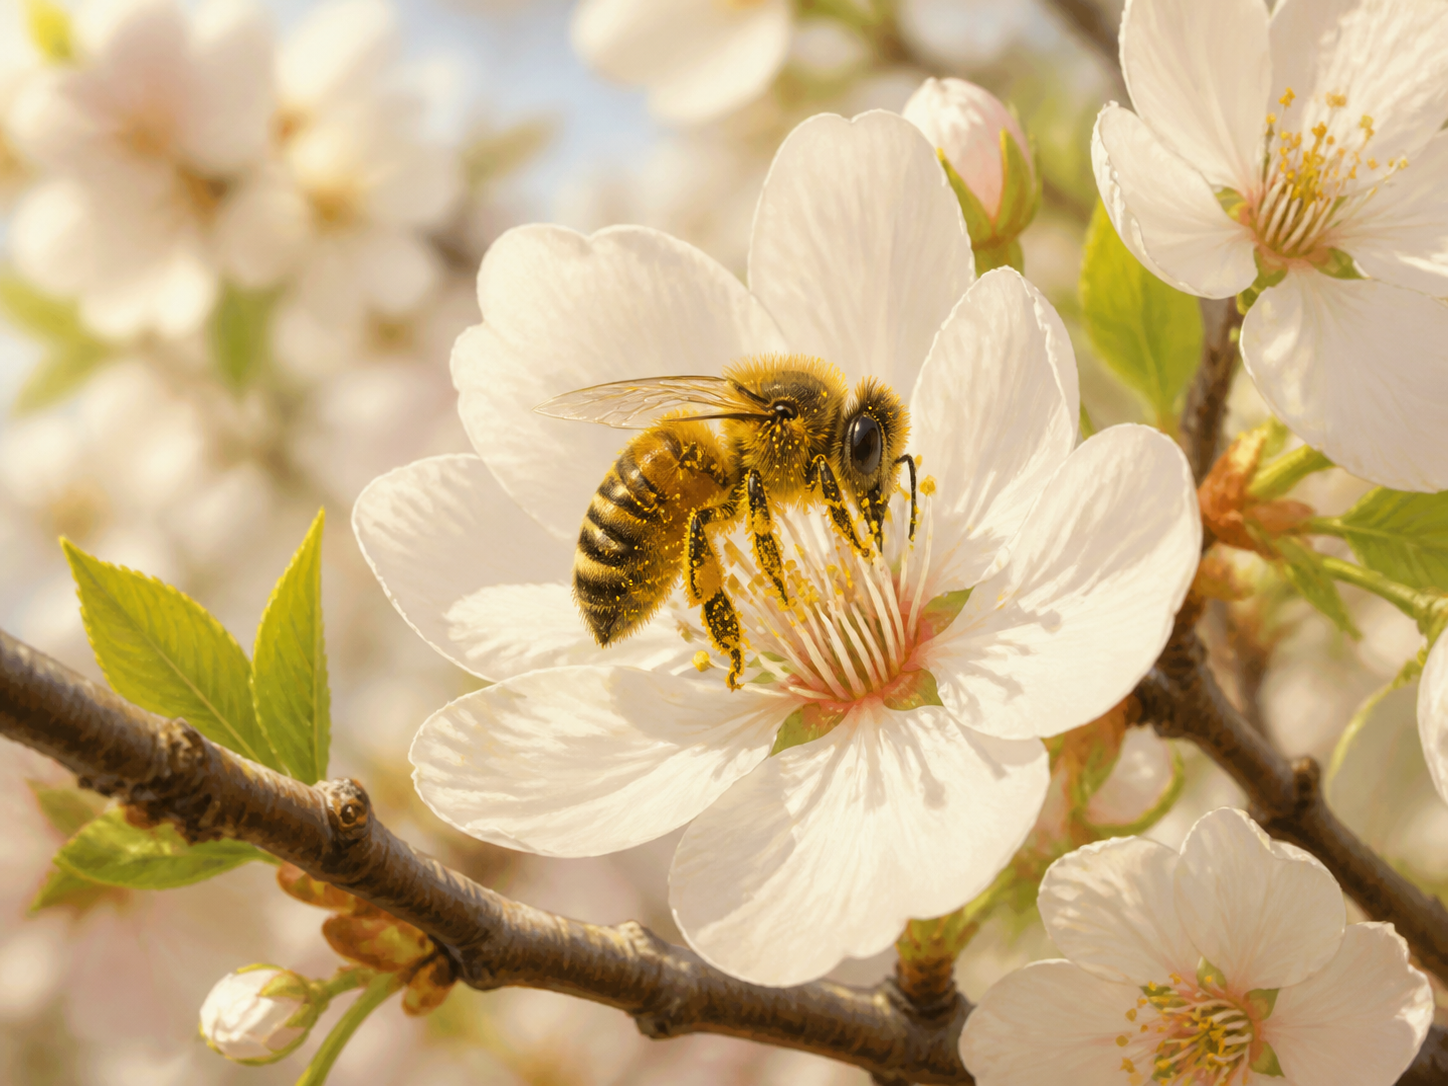
\includegraphics[width=0.58\linewidth]{images/book1/ai/g3-flowers-bee.png}

{\small Pollination in progress: a bee deep in a cherry blossom,
dusted with the \omterm{def:g3:flowers-fruits-seeds:parts}{pollen} it will deliver to the next \omterm{def:g3:flowers-fruits-seeds:parts}{flower}.}
\end{omfigure}

\section{Fruit or not fruit?}

\begin{method}[The seed test]\label{met:g3:flowers-fruits-seeds:test}
To decide whether something from the greengrocer is a \omterm{prop:g3:flowers-fruits-seeds:transform}{fruit} in
the biologist's sense:
\begin{enumerate}
  \item cut it open;
  \item look for \omterm{prop:g3:flowers-fruits-seeds:transform}{seeds} (or a stone, which is a \omterm{def:g2:from-seed-to-plant:seed}{seed} in a hard
        \omterm{def:g1:animals-around-us:covering}{shell});
  \item \omterm{prop:g3:flowers-fruits-seeds:transform}{seeds} inside --- it grew from a \omterm{def:g3:flowers-fruits-seeds:parts}{flower}'s \omterm{def:g3:flowers-fruits-seeds:parts}{pistil}: a \omterm{prop:g3:flowers-fruits-seeds:transform}{fruit}.
        No \omterm{prop:g3:flowers-fruits-seeds:transform}{seeds} anywhere --- it is another part of the \omterm{def:g1:plants-around-us:plant}{plant}:
        \omterm{def:g1:plants-around-us:parts}{root}, \omterm{def:g1:plants-around-us:parts}{stem} or \omterm{def:g1:plants-around-us:parts}{leaf}.
\end{enumerate}
\end{method}

\begin{example}[Surprises at the greengrocer's]\label{ex:g3:flowers-fruits-seeds:surprise}
The \omterm{def:g2:from-seed-to-plant:seed}{seed} test springs surprises. Tomato: full of \omterm{prop:g3:flowers-fruits-seeds:transform}{seeds} --- a
\omterm{prop:g3:flowers-fruits-seeds:transform}{fruit}, whatever the salad bowl says. Cucumber and courgette:
\omterm{prop:g3:flowers-fruits-seeds:transform}{seeds} --- \omterm{prop:g3:flowers-fruits-seeds:transform}{fruits}. Green bean pod: \omterm{prop:g3:flowers-fruits-seeds:transform}{seeds} in a row --- a \omterm{prop:g3:flowers-fruits-seeds:transform}{fruit}.
Carrot: no \omterm{prop:g3:flowers-fruits-seeds:transform}{seeds} --- a \omterm{def:g1:plants-around-us:parts}{root} (\cref{exo:g1:plants-around-us:10}
guessed it). Lettuce: no \omterm{prop:g3:flowers-fruits-seeds:transform}{seeds} --- \omterm{def:g1:plants-around-us:parts}{leaves}. Potato: no \omterm{prop:g3:flowers-fruits-seeds:transform}{seeds} --- a
swollen underground \omterm{def:g1:plants-around-us:parts}{stem}.
\end{example}

\begin{remark}[Kitchen words, science words]\label{rem:g3:flowers-fruits-seeds:words}
In the kitchen, ``\omterm{prop:g3:flowers-fruits-seeds:transform}{fruit}'' means sweet and ``vegetable'' means
savory --- useful for planning dessert, useless for \omterm{def:g1:living-or-not:living}{biology}. The
biologist's word follows the \omterm{def:g2:from-seed-to-plant:seed}{seed} test. Both vocabularies are
fine, as long as you know which one you are speaking.
\end{remark}

\section{Exercises}

\begin{exercise}[$\star$]\label{exo:g3:flowers-fruits-seeds:1}
Name the parts of a \omterm{def:g3:flowers-fruits-seeds:parts}{flower} from the outside in, with each part's
job.
\end{exercise}

\begin{exercise}[$\star$]\label{exo:g3:flowers-fruits-seeds:2}
What is \omterm{def:g3:flowers-fruits-seeds:parts}{pollen}, and where is it found? What is pollination?
\end{exercise}

\begin{exercise}[$\star$]\label{exo:g3:flowers-fruits-seeds:3}
After pollination, what becomes of: (a) the \omterm{def:g3:flowers-fruits-seeds:parts}{petals}? (b) the
\omterm{def:g3:flowers-fruits-seeds:parts}{pistil}? (c) the future \omterm{prop:g3:flowers-fruits-seeds:transform}{seeds} inside it?
\end{exercise}

\begin{exercise}[$\star$]\label{exo:g3:flowers-fruits-seeds:4}
Retell the story of one cherry, from white blossom to red \omterm{prop:g3:flowers-fruits-seeds:transform}{fruit},
in three dated steps.
\end{exercise}

\begin{exercise}[$\star$]\label{exo:g3:flowers-fruits-seeds:5}
Why do cherry growers welcome beehives in the orchard?
\end{exercise}

\begin{exercise}[$\star$]\label{exo:g3:flowers-fruits-seeds:6}
State the \omterm{def:g2:from-seed-to-plant:seed}{seed} test, and apply it to the tomato and the carrot.
\end{exercise}

\begin{exercise}[$\star$]\label{exo:g3:flowers-fruits-seeds:7}
\omterm{prop:g3:flowers-fruits-seeds:transform}{Fruit} or not, by the \omterm{def:g2:from-seed-to-plant:seed}{seed} test: the cucumber, the lettuce, the
green bean pod, the potato?
\end{exercise}

\begin{exercise}[$\star$]\label{exo:g3:flowers-fruits-seeds:8}
Try it: at home, cut open three things from the kitchen and run
the \omterm{def:g2:from-seed-to-plant:seed}{seed} test on each. Which surprised you?
\end{exercise}

\begin{exercise}[$\star\star$]\label{exo:g3:flowers-fruits-seeds:9}
A late frost kills all the blossom on the plum tree in April.
What will the June harvest be, and why? Use
\cref{prop:g3:flowers-fruits-seeds:transform}.
\end{exercise}

\begin{exercise}[$\star\star$]\label{exo:g3:flowers-fruits-seeds:10}
``The apple grows so that we have something nice to eat.'' What
is the apple really for, from the apple tree's point of view?
What lies at its core, and what could each one become? (Recall
\cref{ch:g2:from-seed-to-plant}.)
\end{exercise}
